\documentclass[11pt,fleqn]{article}
\usepackage[cm]{fullpage}
%%AVC PACKAGES
\usepackage{avcgreek}
\usepackage{avcfonts}
\usepackage{avcmath}
\usepackage[numberby=section]{avcthm} % 
\usepackage{qcmacros}
\usepackage{goldstone}
%%MACROS FOR THIS DOCUMENT
\numberwithin{equation}{section}
\usepackage{titlesec}
\titleformat{\section}{\Large\bfseries\mathversion{bold}}{\thesection.}{5pt}{}
% remove header from TOC
\makeatletter
\renewcommand\tableofcontents{%
  \@starttoc{toc}%
}
\makeatother


%%%DOCUMENT%%%
\begin{document}

\section{Diagram notation}

\begin{ntt}
\thmtitle{Particle-hole operators in diagram notation}
In diagram notation, particle-hole operators are written as oriented lines extending from a vertex.
Particle annihilation operators enter the vertex from below, particle creation operators leave the vertex extending upward, and single-excitation operators have both creation and annihilation lines.
Contractions of are represented by joining particle-hole lines with compatible position and orientation.
\begin{align*}
&&
\diagram{
  \node[dot=white,label=above:$p$] (p) at (0,0) {};
  \draw[-<-] (p) to ++(0,-0.5);
}
\equiv
  a_p
&&
\diagram{
  \node[dot=white,label=below:$p$] (p) at (0,0) {};
  \draw[->-] (p) to ++(0,+0.5);
}
\equiv
  a_p^\dagger
&&
\diagram{
  \node[dot=white] (a) at (0,0) {};
  \draw[->-] (a) to ++(0,+0.5) node[above] {$p$};
  \draw[-<-] (a) to ++(0,-0.5) node[below] {$q$};
}
\equiv
  a_p\dg a_q
&&
\diagram{
  \node[dot=white,label=above:$p$] (p) at (0,+0.5) {};
  \node[dot=white,label=below:$q$] (q) at (0,-0.5) {};
  \draw[->-] (q) to (p);
}
\equiv
  \ctr{}{a}{_p}{a} a_p a_q\dg
=
  \d_{pq}
\end{align*}
Note that the vanishing contractions are not expressible in diagram notation.
This has the advantage of simplifying the evaluation of Wick expansions without any loss of generality.
\end{ntt}

\begin{rmk}
\thmtitle{Spin-orbital labels in diagram notation}
When using generic placeholder indices, the spin-orbital labels are dispensed with wherever possible.
The removal of placeholder indices supports the primary objective of diagram notation:
stripping an expression of all extraneous details to reveal its essential information content.
\begin{align*}
&&
\diagram{
  \node[dot=white] (p) at (0,0) {};
  \draw[-<-] (p) to ++(0,-0.5);
}
\mapsto
  a_p
&&
\diagram{
  \node[dot=white] (p) at (0,0) {};
  \draw[->-] (p) to ++(0,+0.5);
}
\mapsto
  a_p^\dagger
&&
\diagram{
  \node[dot=white] (a) at (0,0) {};
  \draw[->-] (a) to ++(0,+0.5);
  \draw[-<-] (a) to ++(0,-0.5);
}
\mapsto
  a_p\dg a_q
&&
\diagram{
  \node[dot=white] (p) at (0,+0.5) {};
  \node[dot=white] (q) at (0,-0.5) {};
  \draw[->-] (q) to (p);
}
\mapsto
  \ctr{}{a}{_p}{a} a_p a_q\dg
\end{align*}
\end{rmk}

\begin{ntt}
\thmtitle{Quasiparticle-quasihole operators in diagram notation}
Diagram notation with respect to $\F$ is expressed in the quasiparticle operator basis, which is indicated by the use of closed- rather than open-circle vertices.
For particles, annihilation operators enter the vertex from below while creation operators leave the vertex extending upward.
For holes, annihilation operators leave the vertex extending downward while creation operators enter from above.
\begin{align*}
&&
\diagram{
  \node[dot] (a) at (0,0) {};
  \draw[-<-] (a) to ++(0,-0.5);
}
\mapsto
  b_a
&&
\diagram{
  \node[dot] (a) at (0,0) {};
  \draw[->-] (a) to ++(0,+0.5);
}
\mapsto
  b_a^\dagger
&&
\diagram{
  \node[dot] (i) at (0,0) {};
  \draw[->-] (i) to ++(0,-0.5);
}
\mapsto
  b_i
&&
\diagram{
  \node[dot] (i) at (0,0) {};
  \draw[-<-] (i) to ++(0,+0.5);
}
\mapsto
  b_i^\dagger
\end{align*}
That is, the hole operator diagrams are rotated by $180^\circ$.
In this basis, there are two possible contractions
\begin{align*}
&&
\diagram{
  \node[dot] (a) at (0,+0.5) {};
  \node[dot] (b) at (0,-0.5) {};
  \draw[->-] (b) to (a);
}
\mapsto
  \ctr{}{b}{_a}{b}  b_ab_b\dg
&&
\diagram{
  \node[dot] (i) at (0,+0.5) {};
  \node[dot] (j) at (0,-0.5) {};
  \draw[-<-] (j) to (i);
}
\mapsto
  \ctr{}{b}{_i}{b}  b_ib_j\dg
\end{align*}
and the single-excitation operator $a_p\dg a_q$ splits into four distinct parts.
\begin{align*}
&&
\diagram{
  \node[dot] (ab) at (0,0) {};
  \draw[->-] (ab) to ++(0,+0.5);
  \draw[-<-] (ab) to ++(0,-0.5);
}
\mapsto
  b_a\dg b_b
=
  a_a\dg a_b
&&
\diagram{
  \node[dot] (ai) at (0,0) {};
  \draw[->-] (ai) to ++(-0.25,+0.5);
  \draw[-<-] (ai) to ++(+0.25,+0.5);
}
\mapsto
  b_a\dg b_i\dg
=
  a_a\dg a_i
&&
\diagram{
  \node[dot] (ia) at (0,0) {};
  \draw[->-] (ia) to ++(-0.25,-0.5);
  \draw[-<-] (ia) to ++(+0.25,-0.5);
}
\mapsto
  b_ib_a
=
  a_i\dg a_a
&&
\diagram{
  \node[dot] (ij) at (0,0) {};
  \draw[-<-] (ij) to ++(0,+0.5);
  \draw[->-] (ij) to ++(0,-0.5);
}
\mapsto
  b_ib_j\dg 
=
  a_i\dg a_j
\end{align*}
\end{ntt}

\begin{dfn}
\thmtitle{Bubble contractions}
A \textit{bubble contraction} is an internal contraction of a single-excitation operator.
\begin{align*}
&&
\diagram{
  \node[dot] (pq) at (0,0) {};
  \draw[->-] (pq) arc (0:360:+0.3) {};
}
\mapsto
  \ctr{}{b}{_i}{b}  b_ib_j\dg
\end{align*}
By convention bubble contractions are defined to represent only hole contractions, since excitation operators have no internal particle contractions.
\end{dfn}


\begin{ex}
The \vac-normal Wick expansion of $a_pa_q\dg$ can be expressed diagram notation as follows.
\begin{align*}
&&
    a_pa_q\dg
  =
  -
    a_q\dg a_p
  +
    \ctr{}{a}{_p}{a} a_pa_q\dg
\hspace{20pt}\leftrightarrow\hspace{20pt}
  \diagram{
    \node[dot=white] (p) at (0,+0.55) {};
    \node[dot=white] (q) at (0,-0.55) {};
    \draw[-<-] (p) to ++(0,-0.5);
    \draw[->-] (q) to ++(0,+0.5);
  }
  =
  -
  \diagram{
    \node[dot=white] (pq) at (0,0) {};
    \draw[->-] (pq) to ++(0,+0.5);
    \draw[-<-] (pq) to ++(0,-0.5);
  }
  +
  \diagram{
    \node[dot=white] (p) at (0,+0.5) {};
    \node[dot=white] (q) at (0,-0.5) {};
    \draw[->-] (q) to (p);
  }
\end{align*}
Note that the operators in a diagram are ordered from top-to-bottom rather than left-to-right [fig~\ref{fig:diagram-example}(a)].
\end{ex}

\begin{ntt}
\thmtitle{Diagram notation for $\vac$- and $\F$-normal-ordered excitation operators}
\vac-normal-ordered excitation operators are expressed in diagram notation as single-excitation operators connected by a line.
$\F$-normal-ordered excitation operators are distinguished from $\vac$-normal-ordered ones by using double-circle vertices.
\begin{align*}
&&
\diagram{
  \node[dot=white] (a1) at (0,0) {};
  \node[dot=white] (a2) at (1,0) {};
  \node (dots) at (1.75,0) {$\cdots$};
  \node[dot=white] (an) at (2.5,0) {};
  \draw (a1)--(a2)--(dots)--(an);
  \draw[->-] (a1) to ++(0,+0.5);
  \draw[->-] (a2) to ++(0,+0.5);
  \draw[->-] (an) to ++(0,+0.5);
  \draw[-<-] (a1) to ++(0,-0.5) coordinate[below left=0.1cm and 0.1cm] (startbrace);
  \draw[-<-] (a2) to ++(0,-0.5);
  \draw[-<-] (an) to ++(0,-0.5) coordinate[below right=0.1cm and 0.1cm] (endbrace);
  \draw[decorate,decoration={brace,mirror}] (startbrace) to node[midway,below=0.1cm] () {\scriptsize{$m$ times}} (endbrace);
}
\mapsto
  \no{a^{p_1}_{q_1}a^{p_2}_{q_2}\cd a^{p_m}_{q_m}}
=
  a^{p_1\cd p_m}_{q_1\cd q_m}
&&
\diagram{
  \node[ddot=white] (a1) at (0,0) {};
  \node[ddot=white] (a2) at (1,0) {};
  \node (dots) at (1.75,0) {$\cdots$};
  \node[ddot=white] (an) at (2.5,0) {};
  \draw (a1)--(a2)--(dots)--(an);
  \draw[->-] (a1) to ++(0,+0.5);
  \draw[->-] (a2) to ++(0,+0.5);
  \draw[->-] (an) to ++(0,+0.5);
  \draw[-<-] (a1) to ++(0,-0.5) coordinate[below left=0.1cm and 0.1cm] (startbrace);
  \draw[-<-] (a2) to ++(0,-0.5);
  \draw[-<-] (an) to ++(0,-0.5) coordinate[below right=0.1cm and 0.1cm] (endbrace);
  \draw[decorate,decoration={brace,mirror}] (startbrace) to node[midway,below=0.1cm] () {\scriptsize{$m$ times}} (endbrace);
}
\mapsto
  \gno{a^{p_1}_{q_1}a^{p_2}_{q_2}\cd a^{p_m}_{q_m}}
=
  \tl{a}^{p_1\cd p_m}_{q_1\cd q_m}
\end{align*}
Here too internal contractions of the diagram are defined to represent hole contractions.
\end{ntt}


\begin{ntt}
\thmtitle{Diagram notation for normal-ordered products of excitation operators}
A pair of excitation operators connected by one or more cross-contractions is implicitly normal-ordered together.
\begin{align*}
\diagram{
% first excitation operator
  \node[dot=white] (a1) at (0,0.5) {};
  \node[dot=white] (a2) at (1,0.5) {};
  \node (dots) at (1.75,0.5) {$\cdots$};
  \node[dot=white] (an) at (2.5,0.5) {};
  \draw (a1)--(a2)--(dots)--(an);
  \draw[->-] (a1) to ++(0,+0.5) coordinate[above left=0.1cm and 0.1cm] (startbrace);
  \draw[->-] (a2) to ++(0,+0.5);
  \draw[->-] (an) to ++(0,+0.5) coordinate[above right=0.1cm and 0.1cm] (endbrace);
  \draw[-<-] (a1) to ++(0,-0.5);
  \draw[-<-] (a2) to ++(0,-0.5);
  \draw[decorate,decoration={brace}] (startbrace) to node[midway,above=0.1cm] () {\scriptsize{$m$ times}} (endbrace);
% second excitation operator
  \node[dot=white] (b1) at (2.5,-0.5) {};
  \node[dot=white] (b2) at (3.5,-0.5) {};
  \node (dots2) at (4.25,-0.5) {$\cdots$};
  \node[dot=white] (bn) at (5.0,-0.5) {};
  \draw (b1)--(b2)--(dots2)--(bn);
  \draw[->-] (b2) to ++(0,+0.5);
  \draw[->-] (bn) to ++(0,+0.5);
  \draw[-<-] (b1) to ++(0,-0.5) coordinate[below left=0.1cm and 0.1cm] (startbrace2);
  \draw[-<-] (b2) to ++(0,-0.5);
  \draw[-<-] (bn) to ++(0,-0.5) coordinate[below right=0.1cm and 0.1cm] (endbrace2);
  \draw[decorate,decoration={brace,mirror}] (startbrace2) to node[midway,below=0.1cm] () {\scriptsize{$n$ times}} (endbrace2);
% connecting line
  \draw[->-] (b1)--(an);
}
\mapsto
  \no{a^{p_1\cd p_m}_{q_1\cd q_m^\hole}a^{r_1^\hole\cd r_n}_{s_1\cd s_n}}
&&
\hspace{15pt}
\diagram{
% first excitation operator
  \node[ddot=white] (a1) at (0,0.5) {};
  \node[ddot=white] (a2) at (1,0.5) {};
  \node (dots) at (1.75,0.5) {$\cdots$};
  \node[ddot=white] (an) at (2.5,0.5) {};
  \draw (a1)--(a2)--(dots)--(an);
  \draw[->-] (a1) to ++(0,+0.5) coordinate[above left=0.1cm and 0.1cm] (startbrace);
  \draw[->-] (a2) to ++(0,+0.5);
  \draw[->-] (an) to ++(0,+0.5) coordinate[above right=0.1cm and 0.1cm] (endbrace);
  \draw[-<-] (a1) to ++(0,-0.5);
  \draw[-<-] (a2) to ++(0,-0.5);
  \draw[decorate,decoration={brace}] (startbrace) to node[midway,above=0.1cm] () {\scriptsize{$m$ times}} (endbrace);
% second excitation operator
  \node[ddot=white] (b1) at (2.5,-0.5) {};
  \node[ddot=white] (b2) at (3.5,-0.5) {};
  \node (dots2) at (4.25,-0.5) {$\cdots$};
  \node[ddot=white] (bn) at (5.0,-0.5) {};
  \draw (b1)--(b2)--(dots2)--(bn);
  \draw[->-] (b2) to ++(0,+0.5);
  \draw[->-] (bn) to ++(0,+0.5);
  \draw[-<-] (b1) to ++(0,-0.5) coordinate[below left=0.1cm and 0.1cm] (startbrace2);
  \draw[-<-] (b2) to ++(0,-0.5);
  \draw[-<-] (bn) to ++(0,-0.5) coordinate[below right=0.1cm and 0.1cm] (endbrace2);
  \draw[decorate,decoration={brace,mirror}] (startbrace2) to node[midway,below=0.1cm] () {\scriptsize{$n$ times}} (endbrace2);
% connecting line
  \draw[->-] (b1)--(an);
}
\mapsto
  \gno{a^{p_1\cd p_m}_{q_1\cd q_m^\hole}a^{r_1^\hole\cd r_n}_{s_1\cd s_n}}
\end{align*}
When excitation operators without cross-contractions are normal ordered together, this is indicated by connecting them with a horizontal dotted line.
\begin{align*}
\diagram{
% first excitation operator
  \node[dot=white] (a1) at (0,0) {};
  \node[dot=white] (a2) at (1,0) {};
  \node (dots) at (1.75,0) {$\cdots$};
  \node[dot=white] (an) at (2.5,0) {};
  \draw (a1)--(a2)--(dots)--(an);
  \draw[->-] (a1) to ++(0,+0.5);
  \draw[->-] (a2) to ++(0,+0.5);
  \draw[->-] (an) to ++(0,+0.5);
  \draw[-<-] (a1) to ++(0,-0.5) coordinate[below left=0.1cm and 0.1cm] (startbrace);
  \draw[-<-] (a2) to ++(0,-0.5);
  \draw[-<-] (an) to ++(0,-0.5) coordinate[below right=0.1cm and 0.1cm] (endbrace);
  \draw[decorate,decoration={brace,mirror}] (startbrace) to node[midway,below=0.1cm] () {\scriptsize{$m$ times}} (endbrace);
% second excitation operator
  \node[dot=white] (b1) at (3.5,0) {};
  \node[dot=white] (b2) at (4.5,0) {};
  \node (dots2) at (5.25,0) {$\cdots$};
  \node[dot=white] (bn) at (6.0,0) {};
  \draw (b1)--(b2)--(dots2)--(bn);
  \draw[->-] (b1) to ++(0,+0.5);
  \draw[->-] (b2) to ++(0,+0.5);
  \draw[->-] (bn) to ++(0,+0.5);
  \draw[-<-] (b1) to ++(0,-0.5) coordinate[below left=0.1cm and 0.1cm] (startbrace2);
  \draw[-<-] (b2) to ++(0,-0.5);
  \draw[-<-] (bn) to ++(0,-0.5) coordinate[below right=0.1cm and 0.1cm] (endbrace2);
  \draw[decorate,decoration={brace,mirror}] (startbrace2) to node[midway,below=0.1cm] () {\scriptsize{$n$ times}} (endbrace2);
% connecting line
  \draw[densely dotted] (an)--(b1);
}
\mapsto
  \no{a^{p_1\cd p_m}_{q_1\cd q_m}a^{r_1\cd r_n}_{s_1\cd s_n}}
&&
\hspace{15pt}
\diagram{
% first excitation operator
  \node[ddot=white] (a1) at (0,0) {};
  \node[ddot=white] (a2) at (1,0) {};
  \node (dots) at (1.75,0) {$\cdots$};
  \node[ddot=white] (an) at (2.5,0) {};
  \draw (a1)--(a2)--(dots)--(an);
  \draw[->-] (a1) to ++(0,+0.5);
  \draw[->-] (a2) to ++(0,+0.5);
  \draw[->-] (an) to ++(0,+0.5);
  \draw[-<-] (a1) to ++(0,-0.5) coordinate[below left=0.1cm and 0.1cm] (startbrace);
  \draw[-<-] (a2) to ++(0,-0.5);
  \draw[-<-] (an) to ++(0,-0.5) coordinate[below right=0.1cm and 0.1cm] (endbrace);
  \draw[decorate,decoration={brace,mirror}] (startbrace) to node[midway,below=0.1cm] () {\scriptsize{$m$ times}} (endbrace);
% second excitation operator
  \node[ddot=white] (b1) at (3.5,0) {};
  \node[ddot=white] (b2) at (4.5,0) {};
  \node (dots2) at (5.25,0) {$\cdots$};
  \node[ddot=white] (bn) at (6.0,0) {};
  \draw (b1)--(b2)--(dots2)--(bn);
  \draw[->-] (b1) to ++(0,+0.5);
  \draw[->-] (b2) to ++(0,+0.5);
  \draw[->-] (bn) to ++(0,+0.5);
  \draw[-<-] (b1) to ++(0,-0.5) coordinate[below left=0.1cm and 0.1cm] (startbrace2);
  \draw[-<-] (b2) to ++(0,-0.5);
  \draw[-<-] (bn) to ++(0,-0.5) coordinate[below right=0.1cm and 0.1cm] (endbrace2);
  \draw[decorate,decoration={brace,mirror}] (startbrace2) to node[midway,below=0.1cm] () {\scriptsize{$n$ times}} (endbrace2);
% connecting line
  \draw[densely dotted] (an)--(b1);
}
\mapsto
  \gno{a^{p_1\cd p_m}_{q_1\cd q_m}a^{r_1\cd r_n}_{s_1\cd s_n}}
\end{align*}
For excitation operators these can obviously be replaced by solid lines, but this distinction will become important when the excitation operators are replaced with $m$-electron operators.
\end{ntt}

\begin{dfn}\label{dfn:m-electorn-operators-antisymmetric-interaction-tensors}
\thmtitle{$m$-electron operators, antisymmetric interaction tensors}
The fundamental components of a diagram (\Cref{dfn:diagram}) are \textit{$m$-electron operators} with \textit{antisymmetric interaction tensors}.
That is, operators of the form
\begin{align*}
&&
  V
=
  \pr{\tfr{1}{m!}}^2
  \sum_{\text{Einstein}}
  \ol{v}_{p_1\cd p_m}^{q_1\cd q_m}
  a^{p_1\cd p_m}_{q_1\cd q_m}
\end{align*}
where the elements of the interaction tensor $\bm{\ol{v}}$ satisfy
$
  \ol{v}_{p_1\cd p_m}^{q_1\cd q_m}
=
  \e_{\pi}
  \ol{v}_{p_{\pi(1)}\cd p_{\pi(m)}}^{q_1\hphantom{_{\pi()}}\cd q_m}
=
  \e_{\pi}
  \ol{v}_{p_1\hphantom{_{\pi()}}\cd p_m}^{q_{\pi(1)}\cd q_{\pi(m)}}
$.
\end{dfn}

\begin{rmk}
\thmtitle{antisymmetrized $m$-electron integrals}
As shown in \Cref{m-electron-operators-ordinary-and-antisymmetrized},
any first-quantized $m$-electron operator
$
  \op{V}=\sum_{i_1<\cd<i_m}\op{v}(i_1,\cd, i_m)
$
can be expanded in Fock space in terms of $m$-electron integrals $v_{p_1\cd p_m}^{q_1\cd q_m}$ as follows.
\begin{align*}
&&
  V
=
  \tfr{1}{m!}
  \sum_{\text{Einstein}}
  v_{p_1\cd p_m}^{q_1\cd q_m}
  a^{p_1\cd p_m}_{q_1\cd q_m}
&&
  v_{p_1\cd p_m}^{q_1\cd q_m}
\equiv
  \int d(1\cd m)\y_{p_1}^*(1)\cd \y_{p_m}^*(m)\op{v}(1\cd m)\y_{q_1}(1)\cd \y_{q_m}(m)
\end{align*}
A simple rearrangement, also shown in \Cref{m-electron-operators-ordinary-and-antisymmetrized}, gives another perfectly valid expression for $V$ in which the interaction tensors are \textit{antisymmetrized $m$-electron integrals} $\ol{v}_{p_1\cd p_m}^{q_1\cd q_m}$.
\begin{align*}
&&
  V
=
  \pr{\tfr{1}{m!}}^2
  \sum_{\text{Einstein}}
  \ol{v}_{p_1\cd p_m}^{q_1\cd q_m}
  a^{p_1\cd p_m}_{q_1\cd q_m}
&&
  \ol{v}_{p_1\cd p_m}^{q_1\cd q_m}
\equiv
  \sum_{\pi\in\mr{S}_m}
  \e_{\pi}
  \ol{v}_{p_1\hphantom{_{\pi()}}\cd p_m}^{q_{\pi(1)}\cd q_{\pi(m)}}
\end{align*}
Therefore, any $m$-electron interaction which can be represented in first-quantization can also be represented in a diagram (\Cref{dfn:diagram}).
\end{rmk}

\begin{dfn}
\thmtitle{Operator element}
For an \textit{$m$-electron operator} $V$, we will use the term \textit{operator element} to refer to a single element of $V$'s interaction tensor times its correspdoning excitation operator, i.e.
$v_{p_1p_2\cdots p_m}^{q_1q_2\cdots q_m}
 a^{p_1p_2\cdots p_m}_{q_1q_2\cdots q_m}\,\text{(no summation)}$
or
$\ol{v}_{p_1p_2\cdots p_m}^{q_1q_2\cdots q_m}
 a^{p_1p_2\cdots p_m}_{q_1q_2\cdots q_m}\,\text{(no summation)}$.
Note that operator elements with antisymmetric interaction tensors are invariant to all permutations of $p_1\cd p_m$ and $q_1\cd q_m$, because the phase factors from the interaction tensor and the excitation operator cancel.
\end{dfn}

\begin{ntt}\label{ntt:goldstone-representation}
\thmtitle{Goldstone operator element}
In Goldstone notation, an element of an operator $V$ is depicted by attaching a label $\bm{v}$ the corresponding excitation operator.
\begin{align*}
\diagram{
  \node[draw] (label) at (-0.7,0) {\bm{v}};
  \node[dot=white] (v1) at (0,0) {};
  \node[dot=white] (v2) at (1,0) {};
  \node (dots) at (1.75,0) {$\cdots$};
  \node[dot=white] (vn) at (2.5,0) {};
  \draw (label)--(v1)--(v2)--(dots)--(vn);
  \draw[->-] (v1) to ++(0,+0.45) node[above] {$p_1$};
  \draw[->-] (v2) to ++(0,+0.45) node[above] {$p_2$};
  \draw[->-] (vn) to ++(0,+0.45) node[above] {$p_m$};
  \draw[-<-] (v1) to ++(0,-0.45) node[below] {$q_1$};
  \draw[-<-] (v2) to ++(0,-0.45) node[below] {$q_2$};
  \draw[-<-] (vn) to ++(0,-0.45) node[below] {$q_m$};
}
\equiv
  \ol{v}_{p_1p_2\cdots p_m}^{q_1q_2\cdots q_m}
  a^{p_1p_2\cdots p_m}_{q_1q_2\cdots q_m}
&&
\hspace{17pt}
\diagram{
  \node[draw] (label) at (-0.7,0) {\bm{v}};
  \node[ddot=white] (v1) at (0,0) {};
  \node[ddot=white] (v2) at (1,0) {};
  \node (dots) at (1.75,0) {$\cdots$};
  \node[ddot=white] (vn) at (2.5,0) {};
  \draw (label)--(v1)--(v2)--(dots)--(vn);
  \draw[->-] (v1) to ++(0,+0.45) node[above] {$p_1$};
  \draw[->-] (v2) to ++(0,+0.45) node[above] {$p_2$};
  \draw[->-] (vn) to ++(0,+0.45) node[above] {$p_m$};
  \draw[-<-] (v1) to ++(0,-0.45) node[below] {$q_1$};
  \draw[-<-] (v2) to ++(0,-0.45) node[below] {$q_2$};
  \draw[-<-] (vn) to ++(0,-0.45) node[below] {$q_m$};
}
\equiv
  \ol{v}_{p_1p_2\cdots p_m}^{q_1q_2\cdots q_m}
  \tl{a}^{p_1p_2\cdots p_m}_{q_1q_2\cdots q_m}
&&
  \text{(no summation)}
\end{align*}
Alternatively, the Goldstone element of an operator is often depicted by using a distinct line style (wavy, zig-zag, etc.) to join the vertices of the excitation operator, instead of attaching a label.
\end{ntt}

\begin{rmk}
\thmtitle{Historical note on Goldstone diagrams}
In the original paper,\footnote{J.~Goldstone, \textit{P.~Roy.~Soc.~A} \textbf{239}, (1957)} Goldstone's diagrams were actually defined in terms of non-antisymmetrized integrals, but this convention has fallen out of favor.
Diagrams using \cref{ntt:goldstone-representation} are more precisely called \textit{antisymmetrized Goldstone diagrams}, also known as \textit{Brandow diagrams}.
\end{rmk}

\begin{ntt}\label{ntt:hugenholtz-representation}
\thmtitle{Hugenholtz operator element}
In Hugenholtz notation, an element of an operator $V$ is depicted as a single labeled vertex with several outgoing and incoming lines.
\begin{align*}
\diagram{
  \node[draw,circle] (label) at (0,0) {\bm{v}};
  \draw[->-] (label.140) -- ++(140:0.5) ++(140:0.2) node {$p_1$};
  \draw[->-] (label.120) -- ++(120:0.5) ++(120:0.2) node {$p_2$};
  \node at (70:0.55) {$\cdot$};
  \node at (80:0.55) {$\cdot$};
  \node at (90:0.55) {$\cdot$};
  \draw[->-] (label.40)  -- ++(40:0.5)  ++(40:0.25)  node {$p_m$};
  \draw[-<-] (label.220) -- ++(220:0.5) ++(220:0.2) node {$q_1$};
  \draw[-<-] (label.240) -- ++(240:0.5) ++(240:0.2) node {$q_2$};
  \node at (270:0.55) {$\cdot$};
  \node at (280:0.55) {$\cdot$};
  \node at (290:0.55) {$\cdot$};
  \draw[-<-] (label.320) -- ++(320:0.5) ++(320:0.25) node {$q_m$};
}
\equiv
  \ol{v}_{p_{\pi(1)}p_{\pi(2)}\cdots p_{\pi(m)}}^{q_{\si(1)}q_{\si(2)}\cdots q_{\si(m)}}
  a     ^{p_{\pi(1)}p_{\pi(2)}\cdots p_{\pi(m)}}_{q_{\si(1)}q_{\si(2)}\cdots q_{\si(m)}}
&&
\hspace{17pt}
\diagram{
  \node[draw,double,circle] (label) at (0,0) {\bm{v}};
  \draw[->-] (label.140) -- ++(140:0.5) ++(140:0.2) node {$p_1$};
  \draw[->-] (label.120) -- ++(120:0.5) ++(120:0.2) node {$p_2$};
  \node at (70:0.55) {$\cdot$};
  \node at (80:0.55) {$\cdot$};
  \node at (90:0.55) {$\cdot$};
  \draw[->-] (label.40)  -- ++(40:0.5)  ++(40:0.25)  node {$p_m$};
  \draw[-<-] (label.220) -- ++(220:0.5) ++(220:0.2) node {$q_1$};
  \draw[-<-] (label.240) -- ++(240:0.5) ++(240:0.2) node {$q_2$};
  \node at (270:0.55) {$\cdot$};
  \node at (280:0.55) {$\cdot$};
  \node at (290:0.55) {$\cdot$};
  \draw[-<-] (label.320) -- ++(320:0.5) ++(320:0.25) node {$q_m$};
}
\equiv
  \ol{v}_{p_{\pi(1)}p_{\pi(2)}\cdots p_{\pi(m)}}^{q_{\si(1)}q_{\si(2)}\cdots q_{\si(m)}}
  \tl{a}^{p_{\pi(1)}p_{\pi(2)}\cdots p_{\pi(m)}}_{q_{\si(1)}q_{\si(2)}\cdots q_{\si(m)}}
&&
  \forall\pi,\si\in\mr{S}_m
\end{align*}
Unlike the Goldstone element, the correspondence between a Hugenholtz element and an algebraic operator element is non-unique, reflecting the symmetry of the operator element with respect to its indices.
However, a Hugenholtz operator can always be directly translated into a Goldstone operator by simply choosing an arbitrary ordering for the outgoing and incoming lines.
\end{ntt}

\begin{dfn}
\thmtitle{Connected pairs, removable sets, connected sets}
A pair of operators is \textit{connected} if they have at least one cross-contraction running between them.
A set $S$ of operators with no connections to operators outside of $S$ is called \textit{removable}.
A set of operators is \textit{connected} if it has no removable subsets.
\end{dfn}

\begin{dfn}
\thmtitle{Degeneracy}
Given a connected product of operators
\begin{align*}
&&
  \sum_{\text{Einstein}}
  \gno{
    \pr{
      v_{uv}^{wx}
      a^{u^{\hole\hole} v}_{w^\ptcl x^{\ptcl\ptcl}}
    }
    \pr{
      w_{yz}^{\a\b}
      a^{y^\ptcl z^{\ptcl\ptcl}}_{\a^{\hole\hole} \b^{\ptcl\ptcl\ptcl}}
    }
    \pr{
      z_{\g\d\e}^{\f\h\th}
      a^{\g\d^{\ptcl\ptcl\ptcl}\e}_{\f\h^{\hphantom{\ptcl\ptcl}}\th}
    }
  }
\hspace{20pt}
  \text{(for example)}
\end{align*}
consider taking the summand and permuting the summed-over index symbols in all possible ways.
The number of index permutations which can be rearranged back into the original summand using only the permutational degrees of freedom of the operator elements is the \textit{degeneracy} of this summand.
The degeneracy of a general product is given by the product of the degeneracies of its connected subsets.
\end{dfn}

\begin{ex}
The following expression has a degeneracy of $2^3=8$
\begin{align*}
&&
  \sum_{\text{Einstein}}
  \gno{
    \pr{
      v_{uv}^{wx}
      a^{uv}_{w^\ptcl x^{\ptcl\ptcl}}
    }
    \pr{
      w_{yz}^{\a\b}
      a^{y^\ptcl z^{\ptcl\ptcl}}_{\a\b}
    }
  }
\end{align*}
because the summand is invariant to $u\leftrightarrow v$ transpositions, simultaneous $\substack{w\leftrightarrow x\\y\leftrightarrow z}$ transpositions, and $\a\leftrightarrow\b$ transpositions.
\end{ex}

\begin{dfn}
\thmtitle{Inequivalent contraction lines}
Lines with vertices on both ends are called \textit{contraction lines}.
Contraction lines with the same orientation that terminate on particle-hole operators at the same vertical level in a diagram are called \textit{inequivalent contraction lines}.
\end{dfn}

\begin{dfn}\label{dfn:diagram}
\thmtitle{Diagram}
A \textit{diagram} is a vertically-arranged [fig~\ref{fig:diagram-example}(a)] visual representation of a product of one or more $m$-electron operators, particle-hole operators, and excitation operators [fig~\ref{fig:diagram-example}(b)] with zero or more contractions.
A diagram translates into an algebraic expression as follows.
\begin{enumerate}
  \item\label{dfn:diagram:item:sum}
  Sum over all unlabeled $m$-electron operator lines (Einstein summation)
  \item\label{dfn:diagram:item:degeneracy-factor}
  Multiply the expression by $D^{-1}$ where $D$ is the degeneracy of the summation
  \item\label{dfn:diagram:item:permutation-factor}
  For each maximal set of inequivalent contraction lines, multiply the expression by an index permutation operator $\op{P}(\a\b\g\cd)$ where $\a\b\g\cd$ are the labels on those lines
\end{enumerate}
The factor $D^{-1}$ will be referred to as the \textit{degeneracy factor} of the diagram.
Note that these rules are reversible: any algebraic term can be translated into a diagram times a scalar factor.
\end{dfn}

\begin{figure}[h!]\label{fig:diagram-example}
\centering
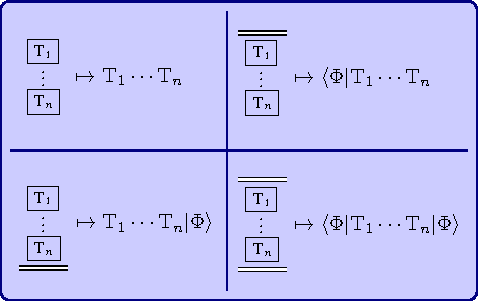
\includegraphics[height=5.7cm]{figs/diagram-ordering.pdf}
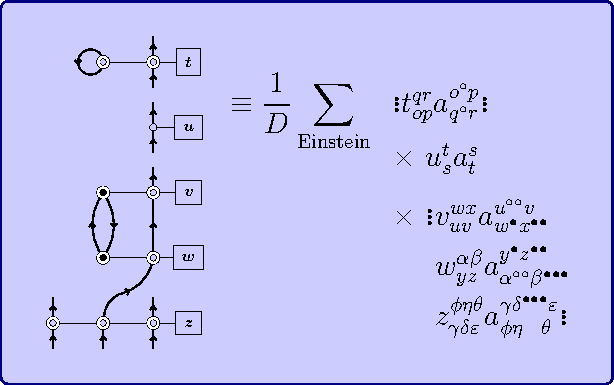
\includegraphics[height=5.7cm]{figs/diagram-example.pdf}
\caption{(a) vertical ordering of a diagram, showing four possible cases of vacuum state bra/ket bookends.
(b)~a~generic example of a diagram, along with its corresponding algebraic term.}
\end{figure}

\begin{ex}
The degeneracy of the product in fig~\ref{fig:diagram-example}(b) is $D=2!2!3!$, so the diagram's degeneracy factor is $\sfr{1}{D}=\sfr{1}{24}$.
\end{ex}

\begin{ex}
Applying the rules of interpretation to a single un-contracted Goldstone operator: 1.~tells us that all lines are summed over, 3.~tells us that the expression has a factor of $\dfr{1}{(m!)^2}$ in front
\begin{align*}
&&
\diagram{
  \node[draw] (label) at (-0.7,0) {\bm{v}};
  \node[dot=white] (v1) at (0,0) {};
  \node[dot=white] (v2) at (1,0) {};
  \node (dots) at (1.75,0) {$\cdots$};
  \node[dot=white] (vn) at (2.5,0) {};
  \draw (label)--(v1)--(v2)--(dots)--(vn);
  \draw[->-] (v1) to ++(0,+0.5);
  \draw[->-] (v2) to ++(0,+0.5);
  \draw[->-] (vn) to ++(0,+0.5);
  \draw[-<-] (v1) to ++(0,-0.5) coordinate[below left=0.1cm and 0.1cm] (startbrace);
  \draw[-<-] (v2) to ++(0,-0.5);
  \draw[-<-] (vn) to ++(0,-0.5) coordinate[below right=0.1cm and 0.1cm] (endbrace);
}
\equiv
  \pr{\tfr{1}{m!}}^2
  \sum_{\substack{p_1\cd p_m\\q_1\cd q_m}}
\diagram{
  \node[draw] (label) at (-0.7,0) {\bm{v}};
  \node[dot=white] (v1) at (0,0) {};
  \node[dot=white] (v2) at (1,0) {};
  \node (dots) at (1.75,0) {$\cdots$};
  \node[dot=white] (vn) at (2.5,0) {};
  \draw (label)--(v1)--(v2)--(dots)--(vn);
  \draw[->-] (v1) to ++(0,+0.45) node[above] {$p_1$};
  \draw[->-] (v2) to ++(0,+0.45) node[above] {$p_2$};
  \draw[->-] (vn) to ++(0,+0.45) node[above] {$p_m$};
  \draw[-<-] (v1) to ++(0,-0.45) node[below] {$q_1$};
  \draw[-<-] (v2) to ++(0,-0.45) node[below] {$q_2$};
  \draw[-<-] (vn) to ++(0,-0.45) node[below] {$q_m$};
}
\equiv&\
  \pr{\tfr{1}{m!}}^2
  \sum_{\text{Einstein}}
  \ol{v}_{p_1p_2\cdots p_m}^{q_1q_2\cdots q_m}
  a^{p_1p_2\cdots p_m}_{q_1q_2\cdots q_m}
\end{align*}
which shows that the diagram is exactly equal to $V$, including the correct summations and the correct scalar factor.
\end{ex}

\begin{ex}
Similarly, for a diagram consisting of a single Hugenholtz operator, we get
\begin{align*}
&&
\diagram{
  \node[draw,circle] (label) at (0,0) {\bm{v}};
  \draw[->-] (label.140) -- ++(140:0.5);
  \draw[->-] (label.120) -- ++(120:0.5);
  \draw[->-] (label.40)  -- ++(40:0.5);
  \node at (70:0.55) {$\cdot$};
  \node at (80:0.55) {$\cdot$};
  \node at (90:0.55) {$\cdot$};
  \draw[-<-] (label.220) -- ++(220:0.5);
  \draw[-<-] (label.240) -- ++(240:0.5);
  \node at (270:0.55) {$\cdot$};
  \node at (280:0.55) {$\cdot$};
  \node at (290:0.55) {$\cdot$};
  \draw[-<-] (label.320) -- ++(320:0.5);
}
\equiv
  \pr{\tfr{1}{m!}}^2
  \sum_{\substack{p_1\cd p_m\\q_1\cd q_m}}
\diagram{
  \node[draw,circle] (label) at (0,0) {\bm{v}};
  \draw[->-] (label.140) -- ++(140:0.5) ++(140:0.2) node {$p_1$};
  \draw[->-] (label.120) -- ++(120:0.5) ++(120:0.2) node {$p_2$};
  \node at (70:0.55) {$\cdot$};
  \node at (80:0.55) {$\cdot$};
  \node at (90:0.55) {$\cdot$};
  \draw[->-] (label.40)  -- ++(40:0.5)  ++(40:0.25)  node {$p_m$};
  \draw[-<-] (label.220) -- ++(220:0.5) ++(220:0.2) node {$q_1$};
  \draw[-<-] (label.240) -- ++(240:0.5) ++(240:0.2) node {$q_2$};
  \node at (270:0.55) {$\cdot$};
  \node at (280:0.55) {$\cdot$};
  \node at (290:0.55) {$\cdot$};
  \draw[-<-] (label.320) -- ++(320:0.5) ++(320:0.25) node {$q_m$};
}
\equiv
  \pr{\tfr{1}{m!}}^2
  \sum_{\text{Einstein}}
  \ol{v}_{p_1p_2\cdots p_m}^{q_1q_2\cdots q_m}
  a^{p_1p_2\cdots p_m}_{q_1q_2\cdots q_m}
\end{align*}
where we have assigned dummy indices of summation in left-to-right order.
\end{ex}



\begin{dfn}
\thmtitle{External and internal lines}
An \textit{external line} is an un-labeled line connected to a single $m$-electron operator, whereas an \textit{internal line} is an un-labeled line connecting one  $m$-electron operator to another.
\end{dfn}

\begin{dfn}
\thmtitle{Equivalent lines}
Two un-labeled lines with the same direction and orientation are called \textit{equivalent} if they are (a) external lines leaving or entering the same $m$-electron operator, or (b) internal lines connected leaving the same $m$-electron operator and entering the same $m$-electron operator.
\end{dfn}

\begin{dfn}
\thmtitle{Equivalent operators}
Two copies of the an $m$-electron operator in a diagram are considered \textit{equivalent} if they are connected to the same set of operators in the same way and their external lines match in orientation. 
\end{dfn}

\begin{drv}
\thmtitle{Counting the degeneracy of a diagram}
Consider a connected diagram.
First, suppose a diagram has no repeated $m$-electron operators.
A permutation of the summation symbols associated with a pair of equivalent lines applies a transposition to the operator symbols within the operators that they leave and enter.
Since this operation can be undone using the permutational degrees of freedom of the operator elements, these permutations contribute to the overall degeneracy.
Permutations of the summation symbols associated with inequivalent lines, on the other hand, permute symbols \ul{between} operators and so cannot be undone using their individual permutational degrees of freedom.
Therefore, if $L$ is the set of lines in the diagram and $\{L_1,\cd, L_g\}$ is the partitioning of $L$ into equivalent lines then the degeneracy of the diagram is the following.
\begin{align}
&&
  D
=
  |L_1|!\cd|L_g|!
\end{align}
%$
%  D
%=
%  |L_1|!\cd|L_g|!\,.$
%Now, suppose the diagram has one or more repeated $m$-electron operators.
%For each pair of equivalent operators, simultaneous transpositions of all of the indices on one of these operators with all of the indices on another also contribute to the degeneracy.
%If $O$ is the full set of operators in the diagram and $\{O_1,\cd,O_h\}$ is the partitioning of $O$ into equivalent operators then the total degeneracy of the diagram is
%\begin{align}
%&&
%  D
%=
%  |L_1|!\cd|L_g|!
%  |O_1|!\cd|O_h|!
%\end{align}
\end{drv}

\begin{dfn}
\thmtitle{Redundancy of a contraction pattern}
Given a connected diagram with a specific contraction pattern, the number of distinct contractions that can be transformed into the original contraction pattern by relabeling summation indices and using the permational degrees of freedom of the operator elements is the \textit{redundancy} $R$ of the pattern.
This is equivalent to the number of contributions in a Wick expansion that are equal to the term with the reference term.
\end{dfn}

\begin{drv}
\thmtitle{Counting the redundancy of a contraction pattern}
Imagine forming the contraction pattern of a connected diagram step-by-step.
First, consider diagram in which all of the contractions have been removed.
Partition the set of lines $L$ in this diagram into equivalent lines $\{L_1,\cd,L_g\}$.
Now, partition each $L_i$ into subsets $\{L_i(0),L_i(1),\cd,L_i(g)\}$ where $L_i(0)$ become external lines and $L_i(j)$ are joined and contracted with $L_j(i)$ in the final diagram.
Note that $|L_i(j)|=|L_j(i)|$ and $|L_i(j)|=0$ unless $L_i$ and $L_j$ have compatible orientations.
The number of equivalent partitionings is therefore
\begin{align*}
&&
  \prod_{i=1}^g
  {|L_i| \choose |L_i(0)|, |L_i(1)|, \ld, |L_i(g)|}
\end{align*}
where $\ds{{n \choose k_1,\ld,k_m}}\equiv\dfr{n!}{k_1!\cd k_m!}$ are multinomial coefficients.
Finally, consider joining together these partitioned sets of equivalent lines into contractions.
For each $L_i(j)$-$L_j(i)$ pair, there are $|L_i(j)|!=|L_j(i)|!$ equivalent ways of contracting the lines, so the total redundancy of the contraction pattern is
\begin{align}
&&\nonumber
  R
=&\
  \prod_{i=1}^g
  {|L_i| \choose |L_i(0)|, |L_i(1)|, \ld, |L_i(g)|}
  \times
  \prod_{i=1}^g
  \prod_{j=i+1}^g
  |S_i(j)|!
\\\intertext{which simplifies to the following.}
&&
  R
=&\
  \prod_{i=1}^g
  \fr{|L_i|!}{|L_i(0)|!}
  \pr{
    \prod_{j=1}^{i-1}
    \fr{1}{|L_i(j)|!}
  }
\end{align}
\end{drv}

%\begin{dfn}
%\thmtitle{Quasi-equivalent lines}
%Two lines with the same direction and orientation that are leaving (entering) the same $m$-electron operator and entering (leaving) two particle-hole operator vertices are called \textit{quasiequivalent}.
%\end{dfn}

\begin{thm}
\thmtitle{Wick's theorem for diagrams}
\thmstatement{The Wick expansion of a product of $m$-electron operators is given by a normal-ordered sum over all unique contracted diagrams, each corresponding to a single algebraic term, without any minus signs or scalar factors.}
\thmproof{
  Clearly, every term in the Wick expansion corresponds to a diagram, and no minus sign is necessary because the phase is defined by the contracted operator string.
  Therefore, it remains to be shown that a single unique diagram is equal to the sum over all redundant contractions corresponding to the pattern.
  That is, the final degeneracy factor $\sfr{1}{D'}$ for a given term must be equal to the redundancy $R$ of its contraction pattern times the original degeneracy factor $\sfr{1}{D}$ of the component diagrams.
  Evaluating the latter, we get
\begin{align*}
  \fr{R}{D}
=
  \prod_{i=1}^g
  \fr{|L_i|!}{|L_i(0)|!}
  \pr{
    \prod_{j=1}^{i-1}
    \fr{1}{|L_i(j)|!}
  }
\times
  \pr{
    \prod_{i=1}^g
    |L_i|!
  }^{-1}
=
  \prod_{i=1}^g
  \fr{1}{|L_i(0)|!}
  \pr{
    \prod_{j=1}^{i-1}
    \fr{1}{|L_i(j)|!}
  }
\end{align*}
  but $\{L_i(0)\}\cup\{L_i(j)\,|\,j<i\}$ is precisely equal the partitioning of the final diagram into equivalent lines, so
\begin{align*}
  D'
=
  \prod_{i=1}^g
  |L_i(0)|!
  \pr{
    \prod_{j=1}^{i-1}
    |L_i(j)|!
  }
=
  \fr{D}{R}
\end{align*}
  which completes the proof.
}
\end{thm}


\begin{dfn}
\thmtitle{Adjacent}
Two that share a vertex are called \textit{adjacent}.
\end{dfn}

\begin{dfn}
\thmtitle{Path}
A sequence of adjacent lines is called a \textit{path}.
Each path has either two external lines, in which case it is an \textit{open path}, or none, in which case it is a \textit{closed path}.
A closed path is also known as a \textit{loop}.
\end{dfn}

\begin{prop}
\thmtitle{Phase factor for a path}
\end{prop}

\begin{cor}
\thmtitle{Phase factor for a loop}
\end{cor}

\begin{cor}
\thmtitle{Phase factor for a completely contracted diagram}
\end{cor}



\end{document}
